\documentclass[UTF8]{ctexart}
\title{电力电子系统建模与仿真作业}
\author{邱哲睿 2016114987\\西南交通大学电气工程学院}
\date{2019年6月1日}
%\usepackage{ctex}
\usepackage[a4paper,top=2.54cm,bottom=2.54cm,left=3.18cm,right=3.18cm]{geometry}
\usepackage{mathtools}
\usepackage{amsmath,amssymb}
\usepackage{extarrows}
\usepackage{graphics}
\usepackage{varwidth}
\usepackage{caption}
\usepackage{subfigure}
\usepackage{svg}
\numberwithin{equation}{section}
\DeclareMathOperator{\dif}{d\!}
\begin{document}
	\begin{titlepage}
		\begin{center}
			\begin{figure}[htbp]
				\centering
				\includegraphics[scale=0.25]{image/School_Name.png}
			\end{figure}
			\begin{figure}[htbp]
				\centering
				\includegraphics[scale=2.7]{image/School_Badge.png}
			\end{figure}
			\phantom{h}
			\newline
			\phantom{h}
			\newline
			\phantom{h}
			\newline
			
			\normalfont \centering
			{\Huge \bfseries 电力电子系统建模与仿真作业1}
			
			\phantom{h}
			\newline
			
			\bigskip
			{\Huge \itshape 邱哲睿}
			
			\bigskip
			\bigskip
			{\Huge 2016114987}
			
			\bigskip
			\bigskip
			{\LARGE 电气(电牵)2016-03班}
			
			\bigskip
			\bigskip
			{\LARGE 2019 年 6 月 1 日}
		\end{center}
		\vspace{\stretch{3}}
	\end{titlepage}
	\maketitle
	\pagestyle{plain}
	\section{建模的作用}
	电力电子装置需要满足静态指标和动态指标的要求,例如负载调整率、变换效率、功率密度、并联模块的不均流度、功率因数。要设计出高品质的装置,不仅需要精心设计主回路,还需要有一个良好的系统控制设计。
	
	\textbf{建模}的作用在于使得人们可以用数学工具对电力电子系统进行分析,从而针对指标要求设计出正确的拓扑,并对电路中的电力电子元件进行合理的控制,使系统达到设计指标。
	
	一个良好的控制系统设计可以显著地提高电力电子装置性能和品质,电力电子系统建模和控制器设计是电力电子系统设计的重要基础。
	\section{反激变换器}
	反激变换器具有结构简单,成本低的特点,同时反激变换器有电气隔离,减少了输入与输出之间的干扰。针对反激变换器存在的诸多缺陷,尤其是为了限制变压器漏电感造成的过电压,本节根据文献,介绍一种电路拓扑及其控制策略——\textbf{非互补有源箝位反激变换器},与传统反激变换器进行对比。
	\subsection{传统反激变换器}
	\subsubsection{传统反激变换器的的劣势}
	传统反激电路工作在硬开关状态下,其有着诸多的缺点,不利于实现开关电源高频化的发展。开关管工作在硬开关时,当其感性关断时,电路中的感性器件如电感、变压器等会产生尖峰电压,频率越高,尖峰电压越大,该电压加在开关管的漏源极两端,对开关管的选型提出了更高的要求,且容易造成开关管击穿;当开关管在较高电压开通时,开关管的内部等效电容储存的能量在开关管内会通过电流的方式释放,开关频率越高,其开通电流的尖峰值也越大,会造成开关管的损耗增大和发热严重的问题;随着开关频率的增大,电路中开关管的 $\frac{\dif v}{\dif t}$ 和 $\frac{\dif i}{\dif t}$ 均会变大,对吸收缓冲电路的设计要求更高,还会导致电磁兼容的问题严重,影响其变换器的工作和周围其他电子产品设备。除此之外,硬开关主要会导致开关损耗的增大,其在开通瞬间,在此区间内,开关管的电流上升,且漏源极间的电压下降,其在关断瞬间,在此区间内,开关管的电流和电压正好与开通瞬间相反,两个区间内电压和电流的交叠产生了开关损耗,频率越高,开关损耗越大。
	
	\newpage
	\subsubsection{传统反激变换器的Simulink仿真模型}
	建立Simulink仿真模型如下图 1 所示\footnote{该仿真模型已上传至https://github.com/VibraniumQ/Flyback\_Compare,下载后请使用MATLAB 2015a以上版本打开}
	
	\begin{figure}[h]
		\centering
		\includegraphics[scale=0.36]{image/tranditional_flyback.png}
		\caption{Simulink仿真模型}
	\end{figure}
	\subsubsection{传统反激变换器的Simulink仿真结果}
	仿真结果如下,以下三幅图均给出变换器稳定工作时两个周期的结果,第一幅图为MOS管门极信号,第二幅图为MOS管漏源极电压,第三幅图为副边二极管电流
	
	\begin{figure}[h]
		\centering
		\includegraphics[scale=0.2]{image/scope.png}
		\caption{开关管漏源极电压}
	\end{figure}

	不难看出,在开关管关断瞬间,漏源极电压存在电压过冲,大约超过稳定后电压值的20\%,如果频率更高,过电压更加严重,可能会造成开关管被击穿。
	
	\subsubsection{传统反激变换器的Simulink仿真结果分析}
	设 $L_m$ 为变压器一次侧励磁电感, $L_k$ 为变压器一次侧漏感, $C_d$ 为开关管谐振电容, $V_{ds}$ 为开关管漏源极电压。
	
	$T_{off1}$阶段为去磁阶段,开关管驱动信号为低电平,变压器一次侧绕组储能结束,MOS管处于截止状态,由于变压器一次侧绕组的励磁电感电流不能突变,其励磁电流在励磁电感在进行续流。此时 $L_k$ 与 $C_d$ 产生LC谐振,,开关管漏源极电压 $V_{ds}$ 发生振荡。
	
	$T_{off2}$阶段,开关管驱动信号依然为低电平,变压器一次侧绕组储存的能量被释放完毕,变压器进行磁复位,二次侧的整流二极管电流  下降到零。变压器一次侧励磁电感 $L_m$ 、漏感 $L_k$ 、电路寄生电阻与开关管电容 $C_d$ 之间发生RLC谐振。
	
	
	\subsection{非互补有源箝位反激变换器}
	\subsubsection{非互补有源箝位反激变换器拓扑介绍}	
	图 3 电路为考虑到变压器漏感以及开关管寄生参数后的非互补有源箝位反激变流器的等效电路拓扑,副边采用肖特基二极管整流方式,图中$L_m$为变压器激磁电感,$L_k$为变压器的漏电感,变压器原副边匝比为 N:1 。$C_{ds\_sw}$代表原边主管的输出电容,$C_{ds\_sa}$代表箝位管输出电容,变压器寄生电容以及副边折算到原边的寄生电容均忽略。
	
	\begin{figure}[h]
		\centering
		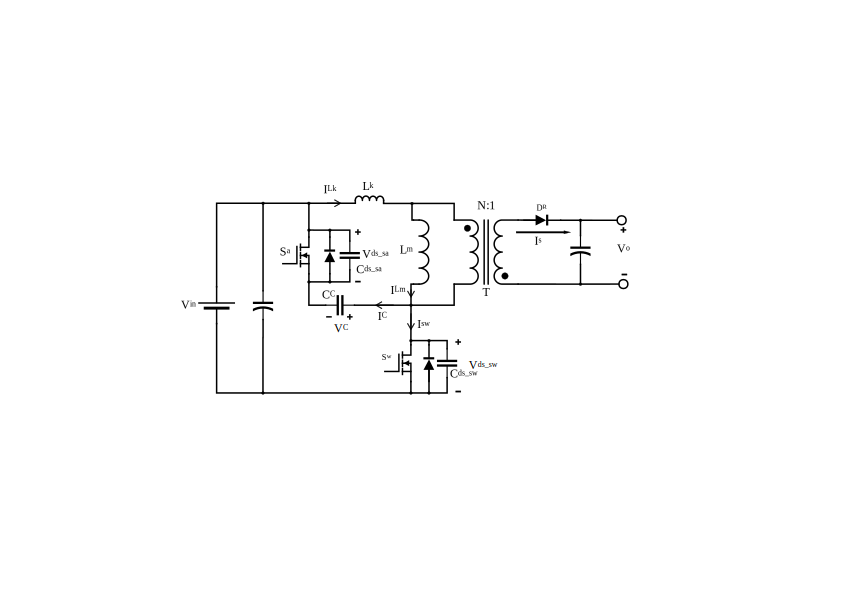
\includegraphics[scale=0.48]{image/NMOS_Clamp.pdf}
		\caption{NMOS箝位}
	\end{figure}

	\subsubsection{非互补有源箝位反激变换器工作原理}
	此处介绍该变换器在激磁电流连续模式下的各个工作阶段。
	
	\begin{figure}[h]
		\centering
		\includegraphics[scale=0.5]{image/mo1.pdf}
		\caption{阶段1 [$T_0 \sim T_1$]}
	\end{figure}
	
	第一阶段[$T_0 \sim T_1$]:在$T_0$时刻,原边漏感电流值上升至激磁电感电流值。理想变压器原边电流值下降为零,因此副边二极管电流也同时下降到零。$S_w$在此前已开通,原边电流流经激磁电感$L_m$线性增长。在此阶段有:
	
	\begin{equation}
	i_{L k}(t)={i}_{L m}(t)=i_{s w}(t)=i_{L m}\left(t_{0}\right)+\frac{V_{i n}}{L_{m}+L_{k}}\left(t-t_{0}\right)
	\end{equation}
	在$T_1$时刻 $S_w$ 关断,阶段 1 结束。
	
	\begin{figure}[h]
		\centering
		\includegraphics[scale=0.6]{image/mo2.pdf}
		\caption{阶段2 [$T_1 \sim T_2$]}
	\end{figure}
	
	第二阶段[$T_1 \sim T_2$]:$T_1$时刻$S_w$关断,原边励磁电流给$S_w$的输出电容$C_{ds\_sw}$充电,而$S_a$的输出电容$C_{ds\_sa}$放电,$V_C$保持不变。在此阶段有:
	
	\begin{equation}
	i_{sw}(t)=\frac{C_{d s\_s w}}{C_{d s\_s w}+C_{d s\_s a}} \cdot {i}_{L m}(t)
	\end{equation}
	\begin{equation}
	i_{c}(t)=\frac{C_{d s\_s a}}{C_{d s\_s w}+C_{d s\_s a}} \cdot {i}_{L m}(t)
	\end{equation}
	\begin{equation}
	V_{d \mathrm{s}\_ s w}(t)=V_{i n}-V_{m} \cos \omega_{0}\left(t-t_{1}\right)-i_{s w}\left(t_{1}\right) \cdot Z_{0} \sin \omega_{0}\left(t-t_{1}\right)
	\end{equation}
	\begin{equation}
	V_{d s\_ s a}(t)=V_{i n}+V_C(t_{1})-V_{d s\_ s w}(t)
	\end{equation}

	其中,$\omega_{0}=\frac{1}{\sqrt{L_{m}\left(C_{d s\_ s w}+C_{d s\_ s a}\right)}}$,$Z_{0}=\sqrt{\frac{L_{m}}{{C_{d s\_s w}}+C_{d s\_ s a}}}$
	
	\begin{figure}[h]
		\centering
		\includegraphics[scale=0.6]{image/mo3.pdf}
		\caption{阶段3 [$T_2 \sim T_3$]}
	\end{figure}
	
	第三阶段[$T_2 \sim T_3$]:当$V_{ds\_sa}$下降为零后,$S_a$体二极管导通。副边整流二极管导通,原边激磁电感两端电压被箝位在$-NV_o$。漏感$L_k$和箝位电容$C_C$谐振。在此阶段有:
	\begin{equation}
	i_{L m}(t)=i_{Lm}\left(t_{2}\right)-\frac{N \cdot V_o}{L_{m}}\left(t-t_{2}\right)
	\end{equation}
	\begin{equation}
	i_{L k}(t)=i_{c}(t)=i_{L m}\left(t_{2}\right) \cos \omega_{1}\left(t-t_{2}\right)-\frac{V c\left(t_{2}\right)-N \cdot V_o}{Z_{1}} \sin \omega_{1}\left(t-t_{2}\right)
	\end{equation}
	\begin{equation}
	V c(t)=N \cdot V_o+\left[V_c\left(t_{2}\right)-N \cdot V_o\right] \cos \omega_{1}\left(t-t_{2}\right)+i_{L k}\left(t_{2}\right) \cdot Z_{1} \sin \omega_{1}\left(t-t_{2}\right)
	\end{equation}
	\begin{equation}
	i_{s}(t)=N \cdot\left[i_{L m}(t)-i_{L k}(t)\right]
	\end{equation}
	其中,$\omega_{1}=\frac{1}{\sqrt{L_{k} C_{C}}}$,$Z_{1}=\sqrt{\frac{L_{k}}{C_{c}}}$
	
	\begin{figure}[h]
		\centering
		\includegraphics[scale=0.5]{image/mo4.pdf}
		\caption{阶段4 [$T_3 \sim T_4$]}
	\end{figure}
	
	第四阶段[$T_3 \sim T_4$]:在$T_3$时刻,漏感电流下降为零,$S_a$截止。副边整流二极管继续导通,原边激磁电感两端电压仍被箝位在$-NV_o$,$S_w$漏源极电压跌至$V_{in}+NV_o$。
	
	\begin{figure}[h]
		\centering
		\includegraphics[scale=0.5]{image/mo5.pdf}
		\caption{阶段5 [$T_4 \sim T_5$]}
	\end{figure}
	
	第五阶段[$T_4 \sim T_5$]:$T_4$时刻$S_a$开通,激磁电感和漏感两端电压被箝位在$-V_C$,$S_w$漏源极电压升至$V_{in}+V_C$。副边整流二极管继续导通,激磁电感两端电压仍被箝位在$-NV_o$,因而漏感两端电压被箝位在$NV_o-V_C$,漏感反向励磁,漏感电流谐振上升。在此阶段有:
	\begin{equation}
	i_{Lk}(t)=i_{c}(t)=-\frac{V c\left(t_{4}\right)-N \cdot V_o}{Z_{1}} \sin \omega_{1}\left(t-t_{4}\right)
	\end{equation}
	\begin{equation}
	V_c(t)=N \cdot V_o+\left[V_c\left(t_{4}\right)-N \cdot V_o\right] \cos \omega_{1}\left(t-t_{4}\right)
	\end{equation}
	$T_5$时刻$S_a$关断,此阶段结束。
	
	\begin{figure}[h]
		\centering
		\includegraphics[scale=0.5]{image/mo6.pdf}
		\caption{阶段6 [$T_5 \sim T_6$]}
	\end{figure}
	
	第六阶段[$T_5 \sim T_6$]:$T_5$时刻$S_a$关断,漏感电流给$S_w$的输出电容放电,同时给$S_a$输出电容$C_{ds\_sa}$充电,箝位电容电压$V_C$保持不变。在此阶段有:
	\begin{equation}
	i_{Lk}(t)=i_{L k}\left(t_{5}\right) \cos \omega_{2}\left(t-t_{5}\right)-\frac{V_c\left(t_{s}\right)-N \cdot V_o}{Z_{2}} \sin \omega_{2}\left(t-t_{5}\right)
	\end{equation}
	\begin{equation}
	i_{s w}(t)=\frac{C_{d s\_s w}}{C_{d s\_s w}+C_{d s\_s a}} \cdot i_{L k}(t)
	\end{equation}
	\begin{equation}
	i_{c}(t)=\frac{C_{d s\_s a}}{C_{d s\_s w}+C_{d s\_s a}} \cdot i_{L k}(t)
	\end{equation}
	\begin{equation}
	V_{d s\_s w}(t)=V_{i n}+N \cdot V_o+\left[V_c\left(t_{5}\right)-N \cdot V_o\right] \cos \omega_{2}\left(t-t_{5}\right)-i_{L k}\left(t_{5}\right) \cdot Z_{2} \sin \omega_{2}\left(t-t_{5}\right)
	\end{equation}
	\begin{equation}
	V_{d s\_s a}(t)=V_{i n}+V_c\left(t_{5}\right)-V_{d s\_s w}(t)
	\end{equation}
	其中,$\omega_{2}=\frac{1}{\sqrt{L_{k}\left(C_{d s\_s w}+C_{d s\_s a}\right)}}$,$Z_{2}=\sqrt{\frac{L_{k}}{C_{d s\_s w}+C_{d s\_s a}}}$
	
	当$V_{d s\_s w}$下降到零时,此阶段结束。
	
	\begin{figure}[h]
		\centering
		\includegraphics[scale=0.5]{image/mo7.pdf}
		\caption{阶段7 [$T_6 \sim T_7$]}
	\end{figure}
	
	第七阶段[$T_6 \sim T_7$]:当$V_{d s\_s w}$下降到零后,$S_w$体二极管导通。漏感$L_k$两端电压为$NV_O-V{in}$,漏感反向电流线性下降,在此阶段有:
	\begin{equation}
	i_{L k}(t)=i_{L k}\left(t_{5}\right)-\frac{V_{i n}-N \cdot V_o}{L_{k}}\left(t-t_{5}\right)
	\end{equation}
	
	原边主管$S_w$必须在漏感电流再次反向之前开通,否则将丢失软开关特性。
	
	\begin{figure}[h]
		\centering
		\includegraphics[scale=0.5]{image/mo8.pdf}
		\caption{阶段8 [$T_7 \sim T_8$]}
	\end{figure}
	
	第八阶段[$T_7 \sim T_8$]:$T_7$时刻$S_w$开通,实现零电压开通。漏感$L_k$两端电压为$V{in}-NV_O$,漏感反向电流继续线性下降,直至为零,然后线性上升。在$T_8$时刻漏感电流等于激磁电流,即$i_{Lk}(t_8) = i_{Lm}(t_8)$,此后漏感电流与激磁电流保持一致线性上升。
	
	\newpage
	\subsubsection{非互补有源箝位反激变换器Simulink仿真模型}
	在仿真模型中,开关管的寄生电容通过调节元件的Snubber capacitance来实现。
	
	\begin{figure}[htbp]
		\centering
		\includegraphics[scale=0.34]{image/new_flyback.png}
		\caption{非互补有源箝位反激变换器Simulink仿真模型}
	\end{figure}
	
	由于参考文献的作者既没有给出详细的电路参数,也没有关于控制策略的详细说明,笔者在多次尝试下,依然无法很好地实现仿真得到合理的结果。
	
	\subsubsection{非互补有源箝位反激变换器总结}
	上文介绍的变换器在保持原有箝位电路不变的基础上提出了一种非互补控制方式。这种非互补有源箝位控制方式实现了原边主管的电压箝位和零电压开通及变压器原边漏感能量回收。同时这种控制方式可以和恒导通时间控制相结合,有效地提高了电路的满载和轻载效率。
	
	这种变换器也存在未解决的问题,例如如何控制箝位管开通点,如何优化高频变压器设计。
	
	\newpage
	\section*{参考文献}
	[1]黄秀成. 非互补有源箝位反激变流器的研究[D].浙江大学,2011.
	
	[2]任于涵. 准谐振反激式同步整流变换器的研究[D].湖南工业大学,2018.
	
	[3]Papanikolaou N P, Tatakis E C. Active voltage clamp in flyback converters operating in CCM mode under wide load variation[J]. IEEE Transactions on industrial electronics, 2004, 51(3): 632-640.
\end{document}